Magnification bias is a well-known weak lensing effect (for a review of weak lensing, we refer the reader to \citealt{BartelmannSchneider01}) that modulates the number density of galaxies in a flux-limited survey. When distant galaxies are magnified by gravitational lenses along the line-of-sight, their observed number per unit area is decreased due to the apparent stretching of space between and around them. At the same time, there is a corresponding increase in their observed brightness. As a consequence, the lensed galaxies are drawn from a fainter source population than the unlensed galaxies, leading to an increase in the number count as galaxies that would normally fall below the limiting magnitude of the survey become detectable with magnification. Through these two competing effects, magnification induces correlations between the galaxies and intervening matter in their foreground, and thus can bias the galaxy-galaxy and galaxy-convergence angular power spectra (see e.g. \citealt{Loverde++08}, \citealt{Ziour++08}, and references contained therein).

In practice, the magnification bias introduces an additional term in the galaxy window function,
\begin{align}
    W^{g}(z)  &\xrightarrow{ } W^{g}(z) + W^{\mu}(z)
\end{align}
which, to first order, is given by
\begin{align}
    W^{\mu}(z) &= (5s-2)\frac{3}{2c} \Omega_{m0} \frac{H_0^2}{H(z)} (1+z) \int_z^{z^{*}} dz^{\prime}g(z^{\prime}) \\
    g(z^{\prime}) &= \frac{\chi(z)(\chi(z^{\prime})-\chi(z))}{\chi(z^{\prime})} \phi(z^{\prime})
\end{align}
%
where $s$ is the slope of the cumulative magnitude function, i.e.\ the response of the number density of the sample to a multiplicative change in brightness at the limiting magnitude of the survey,
\begin{align}
s = \frac{d\log_{10}n(m<m_{\rm lim})}{dm}|_{m=m_{\rm lim}}
\end{align}
This $W^{\mu}$ term in the galaxy window function leads to additional terms in the galaxy-convergence and galaxy-galaxy angular power spectra,
\begin{align}
    C_{\ell}^{\rm \kappa g} &\xrightarrow{} C_{\ell}^{\rm \kappa g} + C_{\ell}^{\kappa \mu} \label{eq:mag-bias-corrections1} \\
    C_{\ell}^{\rm gg} &\xrightarrow{} C_{\ell}^{\rm gg} + 2 C_{\ell}^{\rm g\mu} + C_{\ell}^{\mu\mu} \label{eq:mag-bias-corrections2}
\end{align}

We calculate $s$ by perturbing the observed optical and infrared magnitudes of the imaged objects by a small differential in each direction $\Delta m = \pm 0.01$, then reapplying target selection (as defined in Section~\ref{sec:data:ts}) and measuring the corresponding shifts in the number density of the new LRG samples. Using the finite difference method, we determine $s = 0.999 \pm 0.015$, with the error computed as $\Delta s = (\log_{10}(N) - \log_{10}(N - \sqrt{N}))/\Delta m$. 

We plot the magnification bias corrections\footnote{These terms are calculated using the photometric redshift distribution, so as to avoid assuming a bias evolution model.} as a fraction of the observed spectra (after noise subtraction) in Figure~\ref{fig:mag_bias_frac}. 
% These terms are calculated assuming a \texttt{HaloFit} power spectrum and fiducial bias model $b(z) = 1.6 / D(z)$, and using the photometric redshift distribution.
The corrections to the galaxy-galaxy spectrum are at a level of approximately 5\% over most of the range of scales considered, with 1-2\% increases at edges of the range $\ell < 100$ and $\ell > 900$, while the correction to the cross-spectrum is flat within error bars\footnote{The error bars are dominated by the errors in the cross-spectrum, which become significant at $\ell > 700$.} at 4-5\%. Though the DESI LRG redshift distribution is relatively narrow and peaks at $z < 1$, the high number density and low clustering bias coupled with a steep faint end slope contribute to effects at the level of a few percent, as Figure~\ref{fig:mag_bias_frac} shows.

\begin{figure}
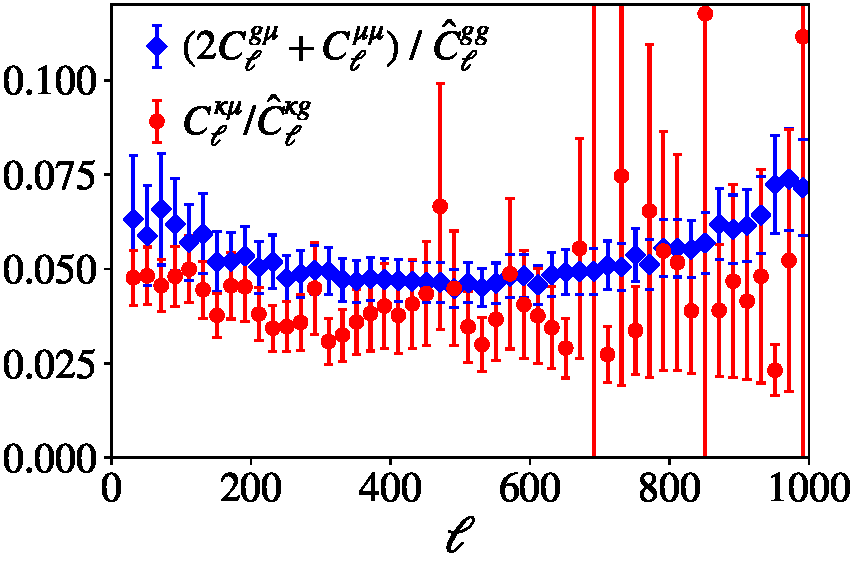
\includegraphics[width=\linewidth,trim={0 1cm 0 0}]{figures/mag_bias_frac.pdf}
\caption{The magnification bias terms of Equations~\ref{eq:mag-bias-corrections1} and \ref{eq:mag-bias-corrections2} as a fraction of the total observed (after subtracting shot noise, in the galaxy-galaxy case) spectra, i.e.\ before correcting for magnification bias. The error bars represent error on the fraction and are dominated by the errors of the denominator.}
\label{fig:mag_bias_frac}
\end{figure}

In all subsequent results, the magnification bias terms have been subtracted from the observed spectra.
